
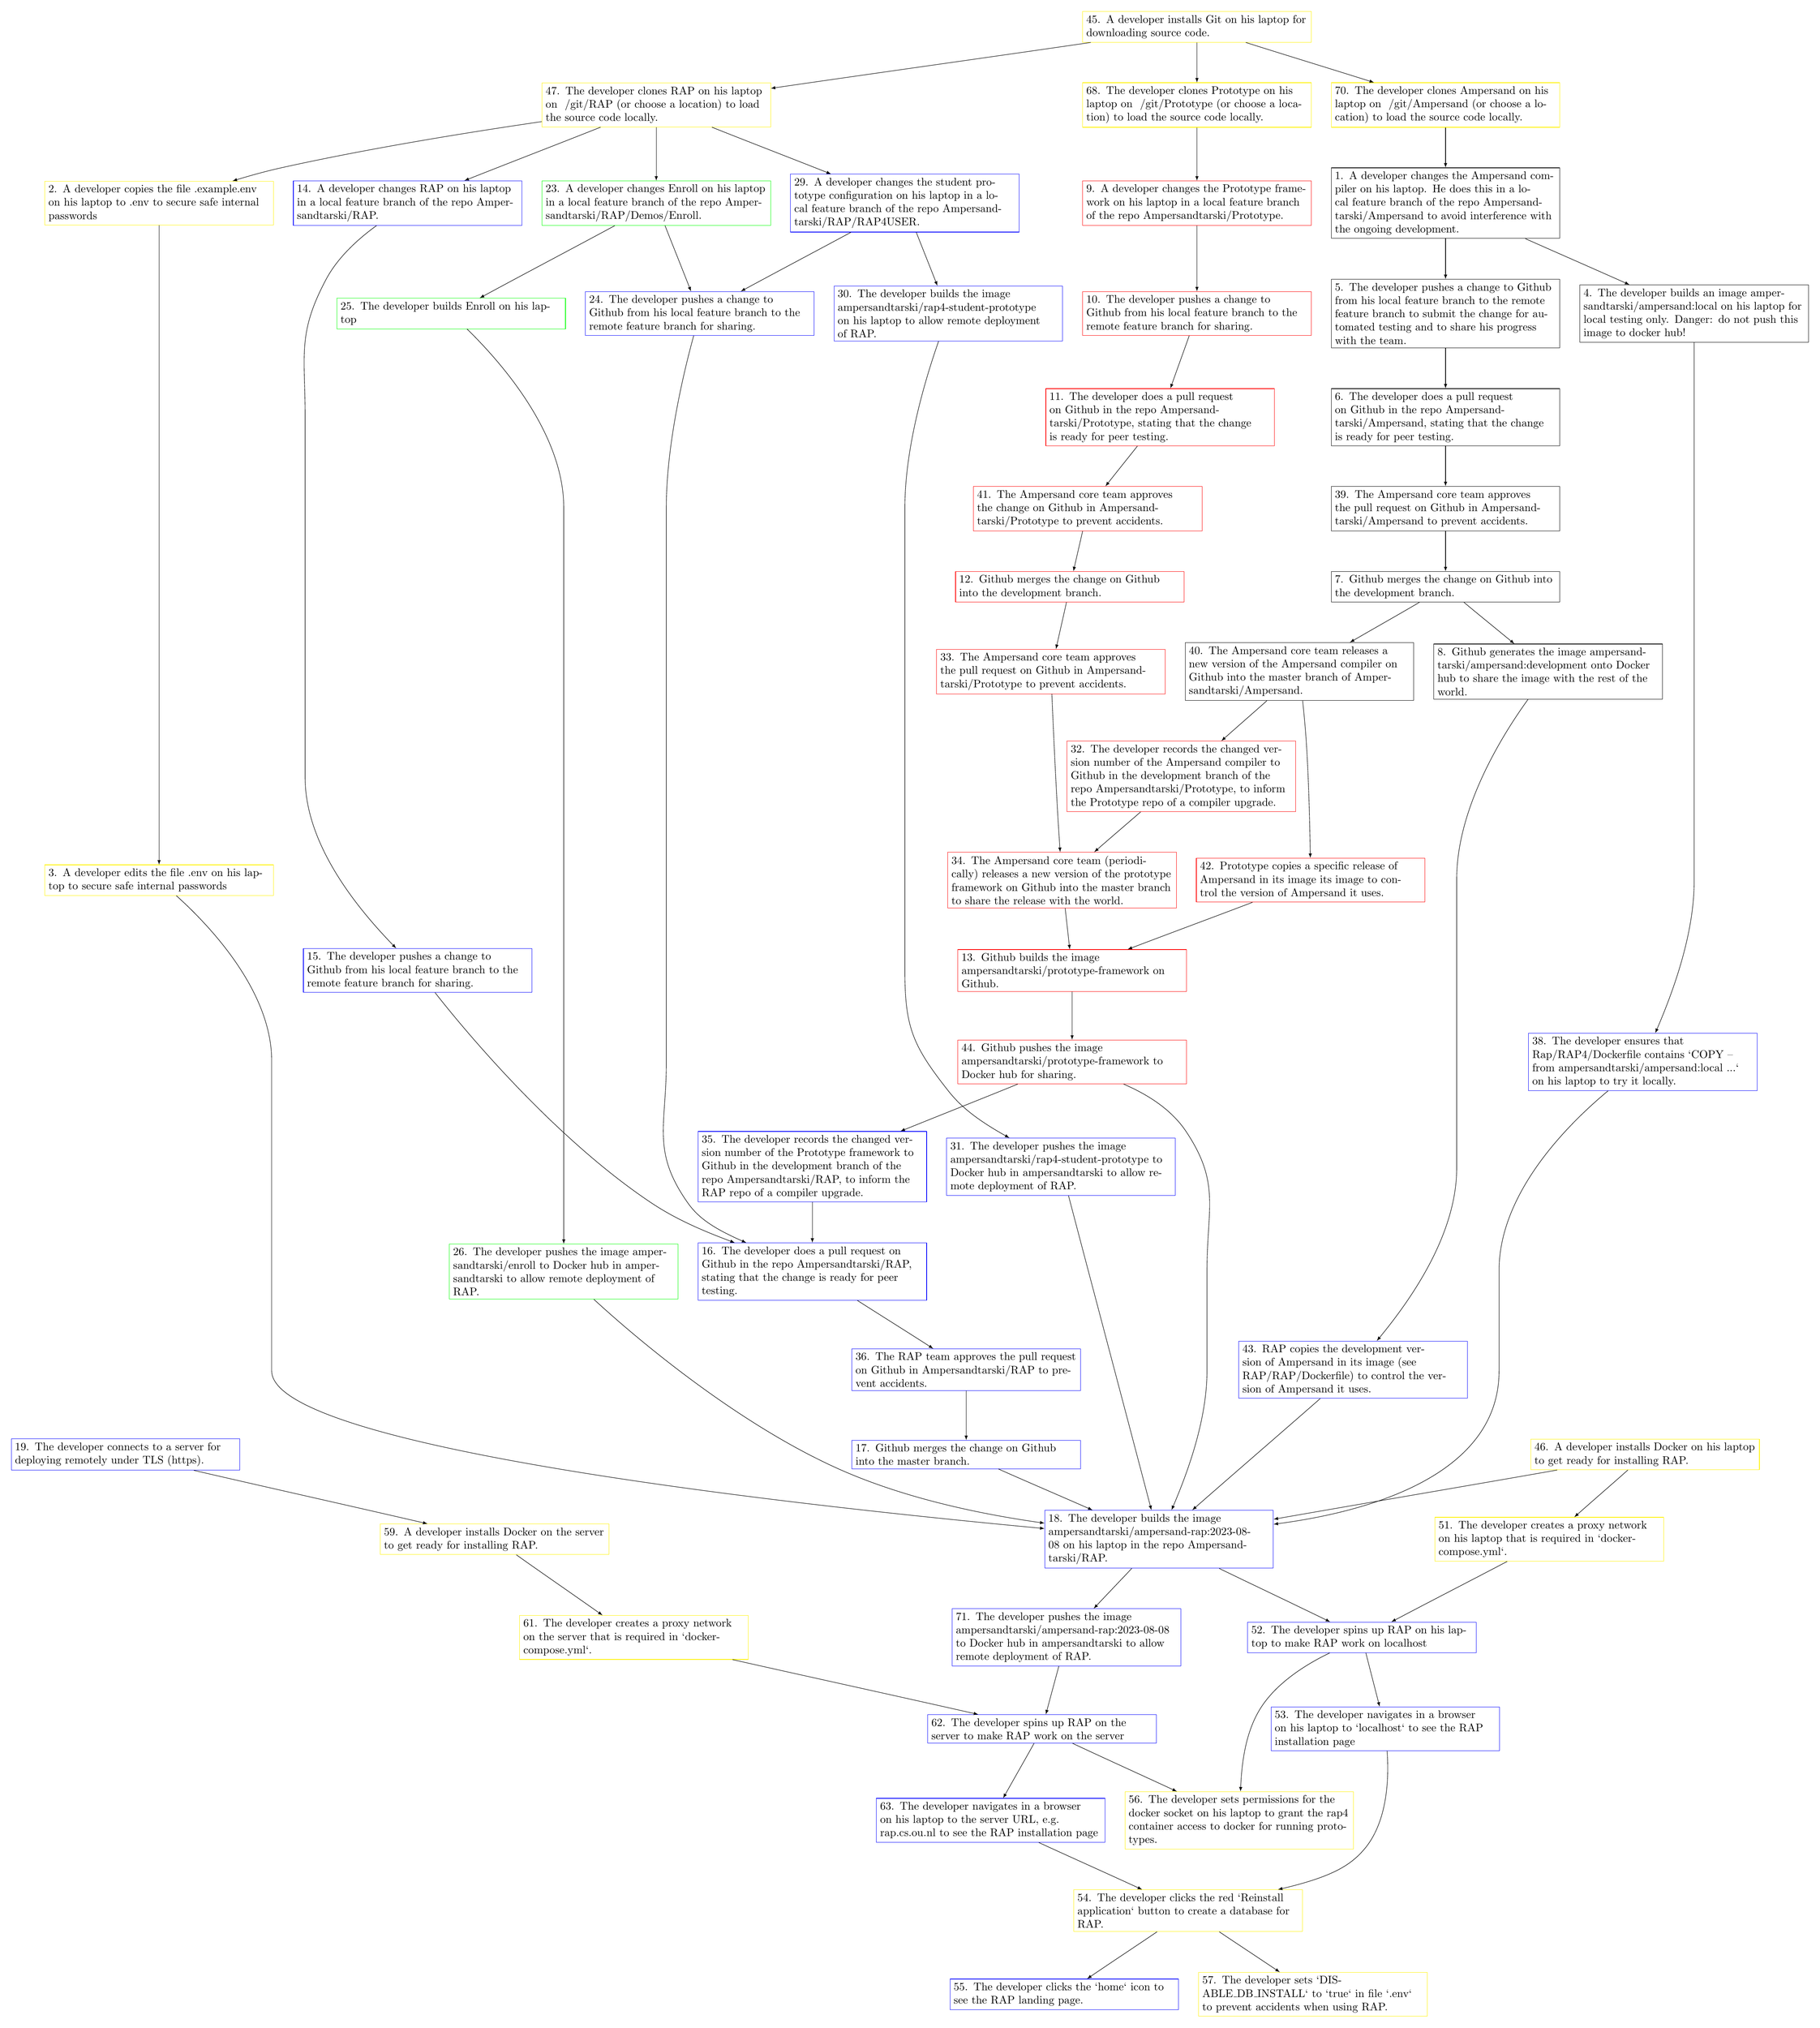
\begin{tikzpicture}[>=latex,line join=bevel,]
%%
\begin{scope}
  \pgfsetstrokecolor{black}
  \definecolor{strokecol}{rgb}{1.0,1.0,1.0};
  \pgfsetstrokecolor{strokecol}
  \definecolor{fillcol}{rgb}{1.0,1.0,1.0};
  \pgfsetfillcolor{fillcol}
  \filldraw (0.0bp,0.0bp) -- (0.0bp,1798.0bp) -- (1612.0bp,1798.0bp) -- (1612.0bp,0.0bp) -- cycle;
\end{scope}
  \node (1) at (1286.5bp,1626.0bp) [draw=black,rectangle,text width=7cm,align=left] {1. A developer changes the Ampersand compiler on his laptop. He does this in a local feature branch of the repo Ampersandtarski/Ampersand to avoid interference with the ongoing development.};
  \node (9) at (1063.5bp,1626.0bp) [draw=red,rectangle,text width=7cm,align=left] {9. A developer changes the Prototype framework on his laptop in a local feature branch of the repo Ampersandtarski/Prototype. };
  \node (14) at (355.5bp,1626.0bp) [draw=blue,rectangle,text width=7cm,align=left] {14. A developer changes  RAP on his laptop in a local feature branch of the repo Ampersandtarski/RAP. };
  \node (23) at (578.5bp,1626.0bp) [draw=green,rectangle,text width=7cm,align=left] {23. A developer changes  Enroll on his laptop in a local feature branch of the repo Ampersandtarski/RAP/Demos/Enroll. };
  \node (4) at (1509.5bp,1527.0bp) [draw=black,rectangle,text width=7cm,align=left] {4. The developer builds an image ampersandtarski/ampersand:local on his laptop  for local testing only. Danger: do not push this image to docker hub!};
  \node (5) at (1286.5bp,1527.0bp) [draw=black,rectangle,text width=7cm,align=left] {5. The developer pushes a change to Github from his local feature branch to the remote feature branch to submit the change for automated testing and to share his progress with the team.};
  \node (2) at (132.5bp,1626.0bp) [draw=yellow,rectangle,text width=7cm,align=left] {2. A developer copies the file .example.env on his laptop to .env to secure safe internal passwords};
  \node (3) at (132.5bp,1019.0bp) [draw=yellow,rectangle,text width=7cm,align=left] {3. A developer edits the file .env on his laptop  to secure safe internal passwords};
  \node (18) at (1029.5bp,428.0bp) [draw=blue,rectangle,text width=7cm,align=left] {18. The developer builds the image ampersandtarski/ampersand-rap:2023-08-08 on his laptop in the repo Ampersandtarski/RAP. };
  \node (38) at (1463.5bp,856.0bp) [draw=blue,rectangle,text width=7cm,align=left] {38. The developer ensures that Rap/RAP4/Dockerfile contains `COPY --from ampersandtarski/ampersand:local ...`  on his laptop  to try it locally.};
  \node (6) at (1286.5bp,1434.0bp) [draw=black,rectangle,text width=7cm,align=left] {6. The developer does a pull request  on Github in the repo Ampersandtarski/Ampersand, stating that the change is ready for peer testing.};
  \node (39) at (1286.5bp,1352.0bp) [draw=black,rectangle,text width=7cm,align=left] {39. The Ampersand core team approves the pull request on Github in Ampersandtarski/Ampersand to prevent accidents.};
  \node (7) at (1286.5bp,1282.0bp) [draw=black,rectangle,text width=7cm,align=left] {7. Github merges the change on Github into the development branch. };
  \node (8) at (1378.5bp,1206.0bp) [draw=black,rectangle,text width=7cm,align=left] {8. Github generates the image ampersandtarski/ampersand:development onto Docker hub  to share the image with the rest of the world.};
  \node (40) at (1155.5bp,1206.0bp) [draw=black,rectangle,text width=7cm,align=left] {40. The Ampersand core team releases a new version of the Ampersand compiler on Github into the master branch of Ampersandtarski/Ampersand. };
  \node (43) at (1203.5bp,580.0bp) [draw=blue,rectangle,text width=7cm,align=left] {43. RAP copies the development version of Ampersand in its image (see RAP/RAP/Dockerfile)   to control the version of Ampersand it uses.};
  \node (10) at (1063.5bp,1527.0bp) [draw=red,rectangle,text width=7cm,align=left] {10. The developer pushes a change to Github from his local feature branch to the remote feature branch for sharing.};
  \node (11) at (1030.5bp,1434.0bp) [draw=red,rectangle,text width=7cm,align=left] {11. The developer does a pull request  on Github in the repo Ampersandtarski/Prototype, stating that the change is ready for peer testing.};
  \node (41) at (965.5bp,1352.0bp) [draw=red,rectangle,text width=7cm,align=left] {41. The Ampersand core team approves the change on Github in Ampersandtarski/Prototype to prevent accidents.};
  \node (12) at (949.5bp,1282.0bp) [draw=red,rectangle,text width=7cm,align=left] {12. Github merges the change on Github into the development branch. };
  \node (33) at (932.5bp,1206.0bp) [draw=red,rectangle,text width=7cm,align=left] {33. The Ampersand core team approves the pull request on Github in Ampersandtarski/Prototype to prevent accidents.};
  \node (13) at (951.5bp,938.0bp) [draw=red,rectangle,text width=7cm,align=left] {13. Github builds the image ampersandtarski/prototype-framework on Github.  };
  \node (44) at (951.5bp,856.0bp) [draw=red,rectangle,text width=7cm,align=left] {44. Github pushes the image ampersandtarski/prototype-framework to Docker hub  for sharing.};
  \node (15) at (364.5bp,938.0bp) [draw=blue,rectangle,text width=7cm,align=left] {15. The developer pushes a change to Github from his local feature branch to the remote feature branch for sharing.};
  \node (16) at (718.5bp,668.0bp) [draw=blue,rectangle,text width=7cm,align=left] {16. The developer does a pull request  on Github in the repo Ampersandtarski/RAP, stating that the change is ready for peer testing.};
  \node (36) at (856.5bp,580.0bp) [draw=blue,rectangle,text width=7cm,align=left] {36. The RAP team approves the pull request on Github in Ampersandtarski/RAP to prevent accidents.};
  \node (17) at (856.5bp,504.0bp) [draw=blue,rectangle,text width=7cm,align=left] {17. Github merges the change on Github into the master branch. };
  \node (52) at (1211.5bp,340.0bp) [draw=blue,rectangle,text width=7cm,align=left] {52. The developer spins up RAP on his laptop  to make RAP work on localhost};
  \node (71) at (946.5bp,340.0bp) [draw=blue,rectangle,text width=7cm,align=left] {71. The developer pushes the image ampersandtarski/ampersand-rap:2023-08-08 to Docker hub in ampersandtarski to allow remote deployment of RAP.};
  \node (19) at (102.5bp,504.0bp) [draw=blue,rectangle,text width=7cm,align=left] {19. The developer connects  to a server  for deploying remotely under TLS (https).};
  \node (59) at (433.5bp,428.0bp) [draw=yellow,rectangle,text width=7cm,align=left] {59. A developer installs Docker on the server  to get ready for installing RAP.};
  \node (24) at (617.5bp,1527.0bp) [draw=blue,rectangle,text width=7cm,align=left] {24. The developer pushes a change to Github from his local feature branch to the remote feature branch for sharing.};
  \node (25) at (394.5bp,1527.0bp) [draw=green,rectangle,text width=7cm,align=left] {25. The developer builds Enroll on his laptop  };
  \node (26) at (495.5bp,668.0bp) [draw=green,rectangle,text width=7cm,align=left] {26. The developer pushes the image ampersandtarski/enroll to Docker hub in ampersandtarski to allow remote deployment of RAP.};
  \node (29) at (801.5bp,1626.0bp) [draw=blue,rectangle,text width=7cm,align=left] {29. A developer changes the student prototype configuration on his laptop in a local feature branch of the repo Ampersandtarski/RAP/RAP4USER. };
  \node (30) at (840.5bp,1527.0bp) [draw=blue,rectangle,text width=7cm,align=left] {30. The developer builds the image ampersandtarski/rap4-student-prototype on his laptop  to allow remote deployment of RAP.};
  \node (31) at (941.5bp,762.0bp) [draw=blue,rectangle,text width=7cm,align=left] {31. The developer pushes the image ampersandtarski/rap4-student-prototype to Docker hub in ampersandtarski to allow remote deployment of RAP.};
  \node (32) at (1049.5bp,1112.0bp) [draw=red,rectangle,text width=7cm,align=left] {32. The developer records the changed version number of the Ampersand compiler to Github in the development branch of the repo Ampersandtarski/Prototype, to inform the Prototype repo of a compiler upgrade.};
  \node (34) at (942.5bp,1019.0bp) [draw=red,rectangle,text width=7cm,align=left] {34. The Ampersand core team (periodically) releases a new version of the prototype framework on Github into the master branch to share the release with the world.};
  \node (35) at (718.5bp,762.0bp) [draw=blue,rectangle,text width=7cm,align=left] {35. The developer records the changed version number of the Prototype framework to Github in the development branch of the repo Ampersandtarski/RAP, to inform the RAP repo of a compiler upgrade.};
  \node (42) at (1165.5bp,1019.0bp) [draw=red,rectangle,text width=7cm,align=left] {42. Prototype copies a specific release of Ampersand in its image its image   to control the version of Ampersand it uses.};
  \node (45) at (1063.5bp,1784.0bp) [draw=yellow,rectangle,text width=7cm,align=left] {45. A developer installs Git on his laptop  for downloading source code.};
  \node (47) at (578.5bp,1714.0bp) [draw=yellow,rectangle,text width=7cm,align=left] {47. The developer clones RAP on his laptop on ~/git/RAP (or choose a location) to load the source code locally.};
  \node (68) at (1063.5bp,1714.0bp) [draw=yellow,rectangle,text width=7cm,align=left] {68. The developer clones Prototype on his laptop on ~/git/Prototype (or choose a location) to load the source code locally.};
  \node (70) at (1286.5bp,1714.0bp) [draw=yellow,rectangle,text width=7cm,align=left] {70. The developer clones Ampersand on his laptop on ~/git/Ampersand (or choose a location) to load the source code locally.};
  \node (46) at (1465.5bp,504.0bp) [draw=yellow,rectangle,text width=7cm,align=left] {46. A developer installs Docker on his laptop  to get ready for installing RAP.};
  \node (51) at (1379.5bp,428.0bp) [draw=yellow,rectangle,text width=7cm,align=left] {51. The developer creates  a proxy network on his laptop  that is required in `docker-compose.yml`.};
  \node (53) at (1232.5bp,258.0bp) [draw=blue,rectangle,text width=7cm,align=left] {53. The developer navigates  in a browser on his laptop to `localhost` to see the RAP installation page};
  \node (56) at (1101.5bp,176.0bp) [draw=yellow,rectangle,text width=7cm,align=left] {56. The developer sets permissions for the docker socket on his laptop  to grant the rap4 container access to docker for running prototypes.};
  \node (54) at (1055.5bp,95.0bp) [draw=yellow,rectangle,text width=7cm,align=left] {54. The developer clicks the red `Reinstall application` button   to create a database for RAP.};
  \node (55) at (944.5bp,20.0bp) [draw=blue,rectangle,text width=7cm,align=left] {55. The developer clicks the `home` icon   to see the RAP landing page.};
  \node (57) at (1167.5bp,20.0bp) [draw=yellow,rectangle,text width=7cm,align=left] {57. The developer sets `DISABLE\_DB\_INSTALL` to `true` in file `.env`   to prevent accidents when using RAP.};
  \node (61) at (558.5bp,340.0bp) [draw=yellow,rectangle,text width=7cm,align=left] {61. The developer creates  a proxy network on the server  that is required in `docker-compose.yml`.};
  \node (62) at (924.5bp,258.0bp) [draw=blue,rectangle,text width=7cm,align=left] {62. The developer spins up RAP on the server  to make RAP work on the server};
  \node (63) at (878.5bp,176.0bp) [draw=blue,rectangle,text width=7cm,align=left] {63. The developer navigates  in a browser on his laptop to the server URL, e.g. rap.cs.ou.nl to see the RAP installation page};
  \draw [->] (1) ..controls (1385.2bp,1582.1bp) and (1414.8bp,1569.2bp)  .. (4);
  \draw [->] (1) ..controls (1286.5bp,1585.9bp) and (1286.5bp,1577.7bp)  .. (5);
  \draw [->] (2) ..controls (132.5bp,1571.2bp) and (132.5bp,1497.3bp)  .. (132.5bp,1435.0bp) .. controls (132.5bp,1435.0bp) and (132.5bp,1435.0bp)  .. (132.5bp,1205.0bp) .. controls (132.5bp,1147.5bp) and (132.5bp,1080.0bp)  .. (3);
  \draw [->] (3) ..controls (176.69bp,979.24bp) and (233.5bp,920.35bp)  .. (233.5bp,857.0bp) .. controls (233.5bp,857.0bp) and (233.5bp,857.0bp)  .. (233.5bp,579.0bp) .. controls (233.5bp,510.45bp) and (695.28bp,459.3bp)  .. (18);
  \draw [->] (4) ..controls (1509.5bp,1467.1bp) and (1509.5bp,1405.6bp)  .. (1509.5bp,1353.0bp) .. controls (1509.5bp,1353.0bp) and (1509.5bp,1353.0bp)  .. (1509.5bp,1018.0bp) .. controls (1509.5bp,973.47bp) and (1493.0bp,924.58bp)  .. (38);
  \draw [->] (5) ..controls (1286.5bp,1488.0bp) and (1286.5bp,1479.6bp)  .. (6);
  \draw [->] (6) ..controls (1286.5bp,1400.1bp) and (1286.5bp,1391.7bp)  .. (39);
  \draw [->] (7) ..controls (1313.1bp,1259.6bp) and (1326.6bp,1248.7bp)  .. (8);
  \draw [->] (7) ..controls (1248.2bp,1259.3bp) and (1228.8bp,1248.4bp)  .. (40);
  \draw [->] (8) ..controls (1335.7bp,1146.8bp) and (1296.5bp,1082.2bp)  .. (1296.5bp,1020.0bp) .. controls (1296.5bp,1020.0bp) and (1296.5bp,1020.0bp)  .. (1296.5bp,761.0bp) .. controls (1296.5bp,705.14bp) and (1260.7bp,649.32bp)  .. (43);
  \draw [->] (9) ..controls (1063.5bp,1592.4bp) and (1063.5bp,1574.1bp)  .. (10);
  \draw [->] (10) ..controls (1052.8bp,1496.4bp) and (1048.0bp,1483.4bp)  .. (11);
  \draw [->] (11) ..controls (1003.0bp,1399.2bp) and (995.3bp,1389.7bp)  .. (41);
  \draw [->] (12) ..controls (944.51bp,1259.3bp) and (941.9bp,1247.9bp)  .. (33);
  \draw [->] (13) ..controls (951.5bp,909.67bp) and (951.5bp,898.28bp)  .. (44);
  \draw [->] (14) ..controls (310.56bp,1593.6bp) and (292.72bp,1577.1bp)  .. (282.5bp,1558.0bp) .. controls (256.43bp,1509.2bp) and (263.5bp,1490.3bp)  .. (263.5bp,1435.0bp) .. controls (263.5bp,1435.0bp) and (263.5bp,1435.0bp)  .. (263.5bp,1111.0bp) .. controls (263.5bp,1053.5bp) and (306.05bp,998.16bp)  .. (15);
  \draw [->] (15) ..controls (411.59bp,877.89bp) and (490.08bp,785.78bp)  .. (573.5bp,730.0bp) .. controls (591.58bp,717.91bp) and (612.43bp,707.44bp)  .. (16);
  \draw [->] (16) ..controls (777.54bp,630.21bp) and (799.17bp,616.73bp)  .. (36);
  \draw [->] (17) ..controls (905.66bp,481.97bp) and (933.53bp,470.05bp)  .. (18);
  \draw [->] (18) ..controls (1111.9bp,388.08bp) and (1146.7bp,371.64bp)  .. (52);
  \draw [->] (18) ..controls (996.85bp,393.17bp) and (987.57bp,383.55bp)  .. (71);
  \draw [->] (19) ..controls (218.97bp,476.96bp) and (302.69bp,458.24bp)  .. (59);
  \draw [->] (23) ..controls (591.72bp,1592.1bp) and (599.26bp,1573.4bp)  .. (24);
  \draw [->] (23) ..controls (509.15bp,1588.4bp) and (461.97bp,1563.6bp)  .. (25);
  \draw [->] (24) ..controls (603.25bp,1475.0bp) and (587.5bp,1409.5bp)  .. (587.5bp,1353.0bp) .. controls (587.5bp,1353.0bp) and (587.5bp,1353.0bp)  .. (587.5bp,855.0bp) .. controls (587.5bp,798.81bp) and (574.24bp,776.01bp)  .. (606.5bp,730.0bp) .. controls (614.86bp,718.08bp) and (626.31bp,708.26bp)  .. (16);
  \draw [->] (25) ..controls (436.9bp,1485.7bp) and (495.5bp,1420.8bp)  .. (495.5bp,1353.0bp) .. controls (495.5bp,1353.0bp) and (495.5bp,1353.0bp)  .. (495.5bp,855.0bp) .. controls (495.5bp,802.7bp) and (495.5bp,742.12bp)  .. (26);
  \draw [->] (26) ..controls (565.13bp,603.95bp) and (654.93bp,529.4bp)  .. (744.5bp,490.0bp) .. controls (798.34bp,466.32bp) and (862.04bp,451.57bp)  .. (18);
  \draw [->] (29) ..controls (725.78bp,1585.1bp) and (691.68bp,1567.1bp)  .. (24);
  \draw [->] (29) ..controls (816.24bp,1588.3bp) and (821.58bp,1575.0bp)  .. (30);
  \draw [->] (30) ..controls (819.93bp,1468.6bp) and (801.5bp,1407.2bp)  .. (801.5bp,1353.0bp) .. controls (801.5bp,1353.0bp) and (801.5bp,1353.0bp)  .. (801.5bp,937.0bp) .. controls (801.5bp,886.38bp) and (809.18bp,869.76bp)  .. (840.5bp,830.0bp) .. controls (851.34bp,816.24bp) and (865.82bp,804.34bp)  .. (31);
  \draw [->] (31) ..controls (963.66bp,677.41bp) and (1002.0bp,532.9bp)  .. (18);
  \draw [->] (32) ..controls (1002.1bp,1070.7bp) and (990.55bp,1060.9bp)  .. (34);
  \draw [->] (33) ..controls (934.39bp,1160.9bp) and (936.36bp,1117.3bp)  .. (938.5bp,1080.0bp) .. controls (938.95bp,1072.1bp) and (939.49bp,1063.6bp)  .. (34);
  \draw [->] (34) ..controls (946.16bp,985.91bp) and (947.17bp,976.97bp)  .. (13);
  \draw [->] (35) ..controls (718.5bp,721.99bp) and (718.5bp,713.79bp)  .. (16);
  \draw [->] (36) ..controls (856.5bp,550.99bp) and (856.5bp,538.93bp)  .. (17);
  \draw [->] (38) ..controls (1392.4bp,796.97bp) and (1334.5bp,736.4bp)  .. (1334.5bp,669.0bp) .. controls (1334.5bp,669.0bp) and (1334.5bp,669.0bp)  .. (1334.5bp,579.0bp) .. controls (1334.5bp,490.67bp) and (1230.2bp,454.35bp)  .. (18);
  \draw [->] (39) ..controls (1286.5bp,1324.2bp) and (1286.5bp,1315.5bp)  .. (7);
  \draw [->] (40) ..controls (1116.3bp,1171.0bp) and (1104.9bp,1161.1bp)  .. (32);
  \draw [->] (40) ..controls (1159.5bp,1168.6bp) and (1160.7bp,1155.7bp)  .. (1161.5bp,1144.0bp) .. controls (1163.6bp,1112.2bp) and (1164.6bp,1075.8bp)  .. (42);
  \draw [->] (41) ..controls (959.17bp,1324.1bp) and (957.1bp,1315.3bp)  .. (12);
  \draw [->] (42) ..controls (1082.3bp,987.29bp) and (1043.7bp,973.02bp)  .. (13);
  \draw [->] (43) ..controls (1144.6bp,528.27bp) and (1099.5bp,489.37bp)  .. (18);
  \draw [->] (44) ..controls (1021.5bp,825.86bp) and (1041.2bp,812.24bp)  .. (1053.5bp,794.0bp) .. controls (1084.8bp,747.35bp) and (1072.5bp,725.19bp)  .. (1072.5bp,669.0bp) .. controls (1072.5bp,669.0bp) and (1072.5bp,669.0bp)  .. (1072.5bp,579.0bp) .. controls (1072.5bp,538.71bp) and (1058.0bp,494.6bp)  .. (18);
  \draw [->] (44) ..controls (875.26bp,824.9bp) and (840.74bp,811.26bp)  .. (35);
  \draw [->] (45) ..controls (888.32bp,1758.4bp) and (776.06bp,1742.7bp)  .. (47);
  \draw [->] (45) ..controls (1063.5bp,1762.7bp) and (1063.5bp,1754.1bp)  .. (68);
  \draw [->] (45) ..controls (1137.4bp,1760.5bp) and (1177.4bp,1748.3bp)  .. (70);
  \draw [->] (46) ..controls (1318.1bp,477.99bp) and (1219.6bp,461.27bp)  .. (18);
  \draw [->] (46) ..controls (1439.1bp,480.29bp) and (1423.9bp,467.2bp)  .. (51);
  \draw [->] (47) ..controls (409.12bp,1689.4bp) and (320.76bp,1675.1bp)  .. (243.5bp,1658.0bp) .. controls (232.17bp,1655.5bp) and (220.29bp,1652.5bp)  .. (2);
  \draw [->] (47) ..controls (495.11bp,1680.8bp) and (451.66bp,1664.1bp)  .. (14);
  \draw [->] (47) ..controls (578.5bp,1683.3bp) and (578.5bp,1669.8bp)  .. (23);
  \draw [->] (47) ..controls (657.22bp,1682.6bp) and (693.27bp,1668.7bp)  .. (29);
  \draw [->] (51) ..controls (1313.7bp,393.34bp) and (1275.7bp,373.85bp)  .. (52);
  \draw [->] (52) ..controls (1217.6bp,315.87bp) and (1221.2bp,301.88bp)  .. (53);
  \draw [->] (52) ..controls (1160.6bp,315.51bp) and (1135.8bp,299.56bp)  .. (1121.5bp,278.0bp) .. controls (1109.0bp,259.07bp) and (1103.9bp,234.05bp)  .. (56);
  \draw [->] (53) ..controls (1235.9bp,214.01bp) and (1234.5bp,174.5bp)  .. (1213.5bp,150.0bp) .. controls (1201.4bp,135.92bp) and (1185.5bp,125.51bp)  .. (54);
  \draw [->] (54) ..controls (1011.2bp,64.845bp) and (990.6bp,51.321bp)  .. (55);
  \draw [->] (54) ..controls (1097.3bp,66.778bp) and (1113.6bp,56.102bp)  .. (57);
  \draw [->] (59) ..controls (471.18bp,401.08bp) and (498.69bp,382.15bp)  .. (61);
  \draw [->] (61) ..controls (711.87bp,305.48bp) and (797.41bp,286.78bp)  .. (62);
  \draw [->] (62) ..controls (974.24bp,234.52bp) and (1006.1bp,220.11bp)  .. (56);
  \draw [->] (62) ..controls (911.39bp,234.2bp) and (902.76bp,219.2bp)  .. (63);
  \draw [->] (63) ..controls (946.54bp,144.63bp) and (977.71bp,130.72bp)  .. (54);
  \draw [->] (68) ..controls (1063.5bp,1683.3bp) and (1063.5bp,1669.8bp)  .. (9);
  \draw [->] (70) ..controls (1286.5bp,1686.7bp) and (1286.5bp,1678.2bp)  .. (1);
  \draw [->] (71) ..controls (936.78bp,303.66bp) and (933.63bp,292.21bp)  .. (62);
%
\end{tikzpicture}
